\section{Software}

\subsection{Generel struktur}

\subsection{Protokol}

\subsection{Eksempler(sensor)}

\subsubsection{Tachometer}

\subsubsection{Lap sensor}

For at initialisere microcontrolleren's comparator skal den sættes op i dens eget status register (ACSR) og i Special Function IO Registret (SFIOR). Man kan vælge flere forskellige inputs til comparatoren - PB2(AIN1) og PB3(AIN0) er henholdsvis ikke-inverterende og inverterende inputs som standard. Alternativt kan hele PORTA bruges til det inverterende og den interne bandgap reference på 2.56 V til det ikke-inverterende.  ACME bit'en i SFIOR enabler ADC multiplexeren, så den styrer hvilket ben på PORTA der bliver brugt. ACBG bit'en enabler bandgap referencen.

\begin{figure}[h]

	\centering
		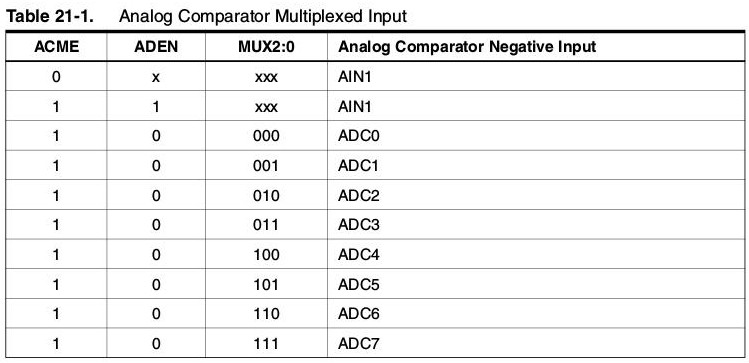
\includegraphics[scale=0.3]{Billeder/Table21-1.jpg}
	\caption{I tabellen kan man se at ACME bit'en lader multiplexeren vælge hvilket ben på PORTA, der er input til comparatorens inverterende ben. Medmindre ADC'en er slået til - så bliver inputtet taget fra PB2(AIN1)}
	\label{fig:ACME}
	
\end{figure}

ikke til at bestemme hvilket ben på PORTA der bliver brugt som input til comparatoren's inverterende ben.  Hvis man ikke bruger PORTA, er PB3 som standard forbundet til det inverterende ben. blev brugt som input for så har man muligheden for at bruge analog til digital converteren uden om comparatoren.

\subsection{AI}

\subsection{GUI}
